\documentclass[a4paper,12pt]{article} % тип документа

% Поля страниц
\usepackage[left=2.5cm,right=2.5cm, top=2cm,bottom=2cm,bindingoffset=0cm]{geometry}
    
%Пакет дял таблиц   
\usepackage{multirow} 
    
%Отступ после заголовка    
\usepackage{indentfirst}

\usepackage{ upgreek }

% Рисунки
\usepackage{subcaption,floatrow,graphicx,calc}
\usepackage{wrapfig}

% Создаёем новый разделитель
\DeclareFloatSeparators{mysep}{\hspace{1cm}}

% Ссылки?
\usepackage{hyperref}
\usepackage[rgb]{xcolor}
\hypersetup{				% Гиперссылки
    colorlinks=true,       	% false: ссылки в рамках
	urlcolor=blue          % на URL
}


%  Русский язык
\usepackage[T2A]{fontenc}			% кодировка
\usepackage[utf8]{inputenc}			% кодировка исходного текста
\usepackage[english,russian]{babel}	% локализация и переносы


% Математика
\usepackage{amsmath,amsfonts,amssymb,amsthm,mathtools, mathrsfs, wasysym}


\begin{document}
\begin{center}
	\footnotesize{ФЕДЕРАЛЬНОЕ ГОСУДАРСТВЕННОЕ АВТОНОМНОЕ ОБРАЗОВАТЕЛЬНОЕ 			УЧРЕЖДЕНИЕ ВЫСШЕГО ОБРАЗОВАНИЯ}\\
	\footnotesize{МОСКОВСКИЙ ФИЗИКО-ТЕХНИЧЕСКИЙ ИНСТИТУТ\\(НАЦИОНАЛЬНЫЙ 			ИССЛЕДОВАТЕЛЬСКИЙ УНИВЕРСИТЕТ)}\\
	\footnotesize{ФАКУЛЬТЕТ ОБЩЕЙ И ПРИКЛАДНОЙ ФИЗИКИ\\}
	\hfill \break
	\hfill\break
	\hfill\break
	\hfill \break
	\hfill \break
	\hfill \break
	\hfill \break
	\hfill \break
	\hfill \break
	\hfill \break
	\hfill \break
	\hfill \break
	\hfill \break
	\hfill \break
	\large{Лабораторная работа № 5.10.1 \\\textbf{Электронный парамагнитный резонанс.}}\\
	\hfill \break
	\hfill \break
	\hfill \break
	\begin{flushright}
		Серебренников Даниил\\
		Группа Б02-826м
	\end{flushright}
	\hfill \break
	\hfill \break
	\hfill \break
	\hfill \break
	\hfill \break
	\hfill \break
	\hfill \break
	\hfill \break
	\hfill \break
	\hfill \break
	\hfill \break
\end{center}
\begin{center}
	Долгопрудный, 2020 г.
\end{center}
\thispagestyle{empty}
\newpage
	\textbf{Цель работы:} Исследуется электронный парамагнитный резонанс в молекуле ДФПГ, определяется $g$-фактор электрона, измеряется ширина ЭПР.

\section{Теоретическая часть}
	Энергетический уровень электрона в пристутсвии магнитного поля с индукцией $B$ расщепляется на подуровня, расстояние между которыми равно 
	\begin{equation}
		\label{eq:dE}
		\Delta E = E_2 - E_1 = 2\mu B.
	\end{equation}
	Здесь $\mu$ -- абсолютная величина проекции магнитного момента на направление поля.
	
	Между этими двумя уровнями возможны переходы. Эти переходы могут возбуждаться внешним выскочастотным электромагнитным полем, если оно имеет нужную частоту и нужное направление.
	
	Резонансное значение частоты определяется из очевидной формулы:
	\begin{equation}
		\label{eq:resonans_omega}
		\hbar \omega_0 = \Delta E.
	\end{equation}

	При переходе с нижнего на верхний уровень энергии электрон поглощает квант электромагнитной энергии, а при обратном переходе такой же квант излучается. Возбуждение электронных резонансных переходов электромагнитным полем, имеющим частоту, определяемую формулой~(\ref{eq:resonans_omega}), носит название электронного парамагнитного резонанса (ЭПР).
	
	В настоящей работе необходимо получить сигнал ЭПР на кристаллическом дифенилпикрилгидразиле (ДФПГ) и определить значение $g$-фактора для электрона. Как известно, связь между магнитным моментом $\upmu$ электрона и его механическим моментом $\mathbf{M}$ выражается через гиромагнитное отношение $\gamma$ с помощью формулы
	\begin{equation}
		\label{eq:gyromagnit}
		\upmu = \gamma \mathbf{M}.
	\end{equation}

	Используя соотношения (\ref{eq:dE})-(\ref{eq:gyromagnit}), нетрудно получить выражение для $g$-фактора через определяемые экспериментально величины:
	\begin{equation}
		\label{eq:g-faktor}
		\tag{$\star$}
		g = \frac{\hbar \omega_0}{\mu_\text{Б}B}.
	\end{equation}

\newpage
\section{Экспериментальная установка}
	Образец (порошок ДФПГ) в стеклянной ампуле помещяется внутрь катушкииндуктивнсоти входящей в состав колебательного контура. Входящий в состав контура конденсатор состоит из двух платсин, разделенных воздушным зазором, одна из пластин может перемещаться поворотом штока. Колебания в контуре возбуждаются антенной, соединённой с генератором частоты (ВЧ) Г4-116. Амплитуда колебаний поля в катушке индуктивности измеряется по наводимой в петле связи ЭДС индукции. Высокочастотные колебания ЭДС индукции в приёмном контуре детектируются диодом, измеряемая при помощи осциллографа низкочастотная огибающая этого сигнала пропорциональна квадрату амплитуды колебаний поля в катушке.
	\begin{figure}[h!]
		\begin{floatrow}
			\ffigbox[\FBwidth]{\caption{Схема установки.}\label{fig:ustanovka}}%
			{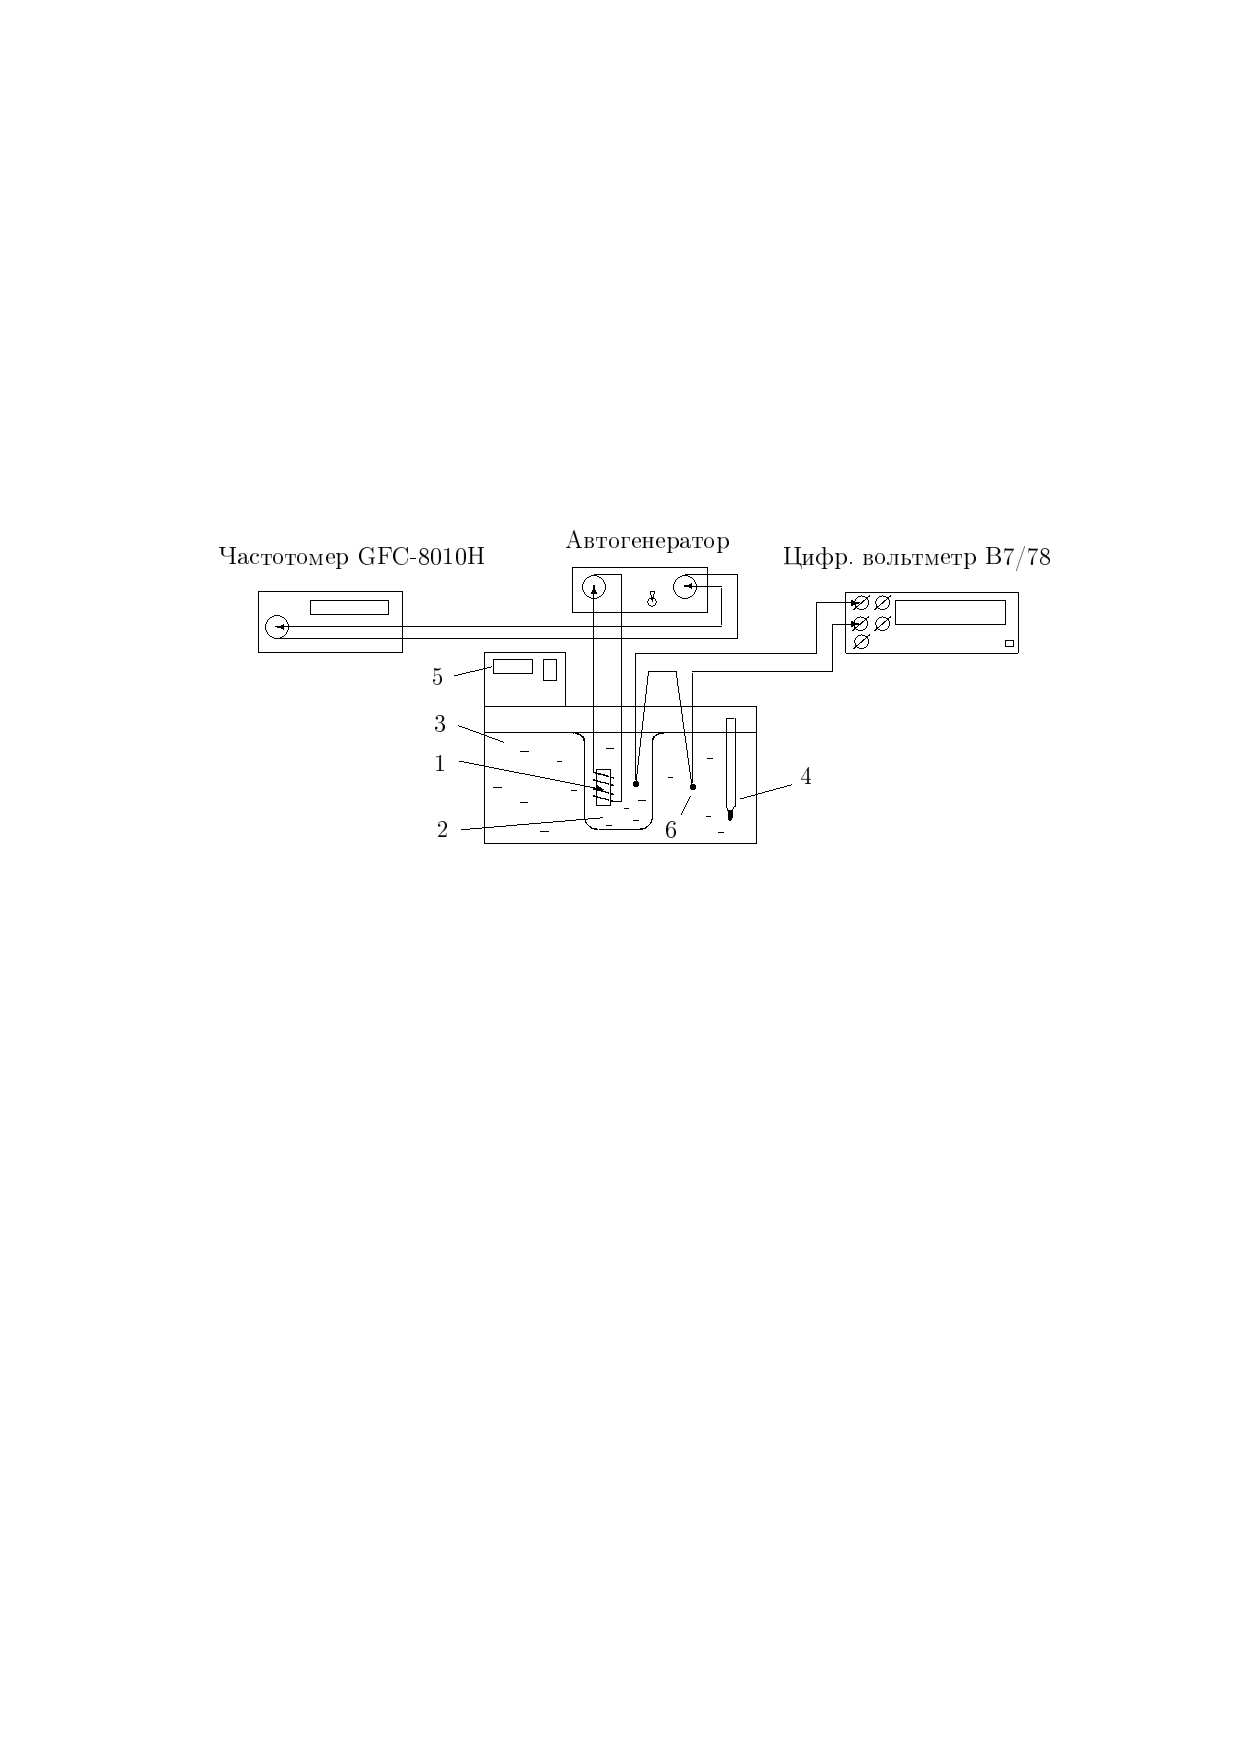
\includegraphics[scale=1]{ustanovka.pdf}}    
		\end{floatrow}
	\end{figure}
	
	Постоянной магнитное поле создаётся пропусканием тока от источника постоянного тока через основные катушки. При этом при помощи вольтметра измеряется падение напряжения на резисторе в цепи основных катушек. Переменное поле небольшой амплитуды создаётся подачей на модуляционные катушки напряжения с регулируемого трансформатора ЛАТР. Для измерения амплитуды колебаний переменного поля используется пробная катушка известной геометрии, подключенная к вольтметру.
	
	
	
	\newpage
	\section{Обработка результатов}
		Настроим генератор на частоту колебательного конутра. Получаем резонансную частоту:
		\begin{equation*}
			f_0 = (128,97 \pm 0,01) \ \text{Мгц}.
		\end{equation*}
		Запишем также частоты $f_{+1/2}$ и $f_{-1/2}$, при которых амплитуда сигнала падает в два раза:
		\begin{equation*}
			f_{-1/2} = (128,75\pm 0,01) \ \text{Мгц}, \ f_{+1/2} = (129,2 \pm 0,01)\ \text{Мгц},
		\end{equation*}
		откуда добротность:
		\begin{equation*}
			Q = (286,5 \pm 0,5)
		\end{equation*}
	
		Подберем величину постоянного магнитного поля в катушках так, чтобы наблюдался сигнал резонанского поглощения. Для этого подадим на катушки достаточное напряжение.
		
		Для более точной настройки и определения ширины линии резонасного поглощения будем наблюдать сигнал в $XY$-режиме. Запишем значение напряжения на резисторе в цепи основных катушек:
		\begin{equation*}
			U_0 = (92,7 \pm 0,1) \ \text{мВ}.
		\end{equation*}
	
		Определим ширину линии ЭПР (полуширина на на полувысоте линии резонасного поглощения):
		\begin{equation*}
			\Delta B = \frac{A_{1/2}}{A_{\text{полн}}}B_\text{мод},
		\end{equation*}
		где $A_\text{полн}$ -- полный размах модулирующего поля, $A_{1/2}$ -- ширина кривой на полувысоте, $B_\text{мод}$ -- амплитуда модулирующего поля.
		\begin{equation*}
			\begin{gathered}
				A_\text{полн} = (8,2 \pm 0,1 ) \ \text{дел}, \ A_{1/2} = (1,5 \pm 0,1) \ \text{дел} \\
				B_\text{мод} = \sqrt{2} \frac{2\varepsilon}{\pi^2d^2N\nu},
			\end{gathered}
		\end{equation*}
		где $\varepsilon$ -- ЭДС индукции при внесении пробной катушки, $N$ -- число витков катушки, $d$ -- диаметр катушки, $\nu$ -- частота модулирующего напряжения.
		
		Имеем:
		\[\boxed{\Delta B = (0,15 \pm 0,01) \ \text{мТл}}.\]
		
		Определим связь между падением напряжения на резисторе в цепи основных катушек и магнитным полем в центре магнита. Для этого построим график (рис.~\ref{fig:E(U)}) зависимости ЭДС индукции в пробной катушке от падения напряжения в цепи основных катушек.
		
		\begin{figure}[h!]
			\begin{floatrow}
				\ffigbox[\FBwidth]{\caption{Зависимость $\varepsilon = \varepsilon(U)$.}\label{fig:E(U)}}%
				{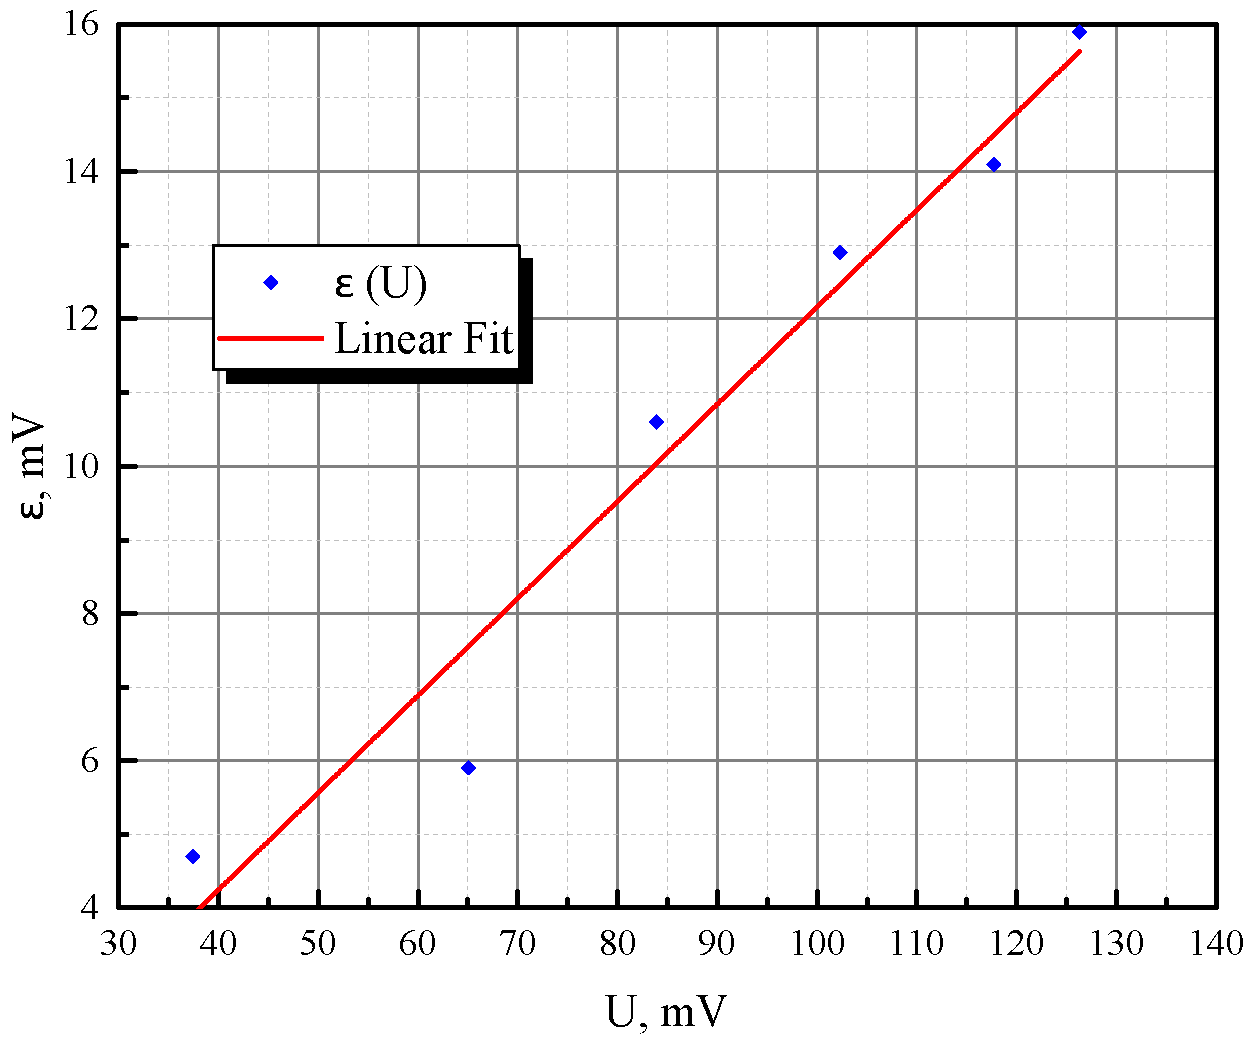
\includegraphics[scale=0.5]{graph.pdf}}    
			\end{floatrow}
		\end{figure}
		\floatsetup[table]{capposition=top}	
		\begin{table}[H]
			\caption{$\varepsilon (U) = aU + b$.}
			\label{tab:P}
			\begin{tabular}{|c|c|}
				\hline
				$a$ & $b$, мВ \\ \hline
				$0,132 \pm 0,001 $   & $-1,03 \pm 0,01$       \\ \hline
			\end{tabular}
		\end{table}
		
		При $U=U_0$ получаем значение $\varepsilon_0 = (11,0 \pm 0,1)$ мВ. Формула для $g$-фактора имеет следующий вид:
		\begin{equation*}
			g = \frac{hf_0}{\mu_BB_0} = 2,0 \pm 0,1,
		\end{equation*}
		где
		\begin{equation*}
			B_0 = \frac{\varepsilon_0}{2\pi\nu N \frac{\pi d^2}{4}} = (4,45 \pm 0,05) \text{мТл}.
		\end{equation*}
		

\newpage
\section{Обсуждение результатов и выводы}
	В настоящей работе был экспериментально проверен эффект парамагнитного резонанса. Определена добротность колебательного окнтура. Найдена полуширина линии резонасного поглощения. Получена завивисимость ЭДС индукции на катушках от напряжения на резисторе. Также найдет $g$-фактор свободного электрона в веществе. Результаты по порядку величины в пределах погрешности совпали с табличными.
	
	Заметим, что $g$-фактор, полученный из электронного парамагнитного резонанса в ДФПГ, всего на десятые доли процента отличается от $g$-фактора свободного электрона. Это обсуловлено чисто чисто спиновым характером магнетизма в ДФП: парамагнитный резонанс на неспаренных электронах происходит почти как на свободных частицах.	


\end{document}